\section{Results}
\label{sec:results}

\begin{figure}[htbp]
	\centering
	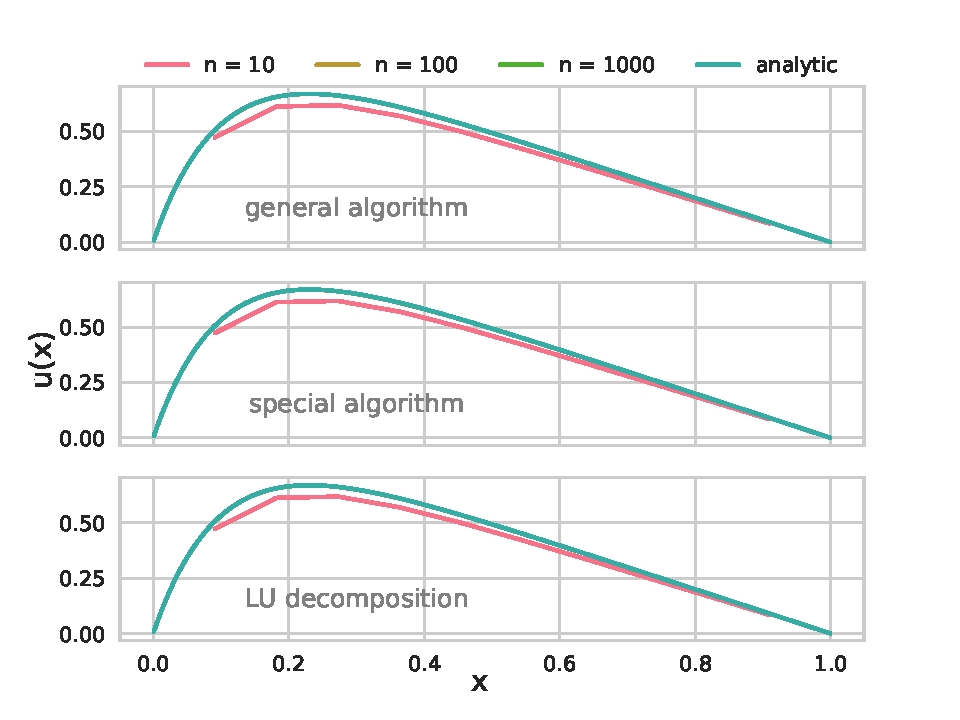
\includegraphics[width=\textwidth]{all_matrix_compare.pdf}
	\caption{Here we show the relative error as a function of Monte Carlo cycles in the case of the 2x2 Ising lattice.}
	\label{fig:compare}
\end{figure}

\begin{figure}[htbp]
	\centering
	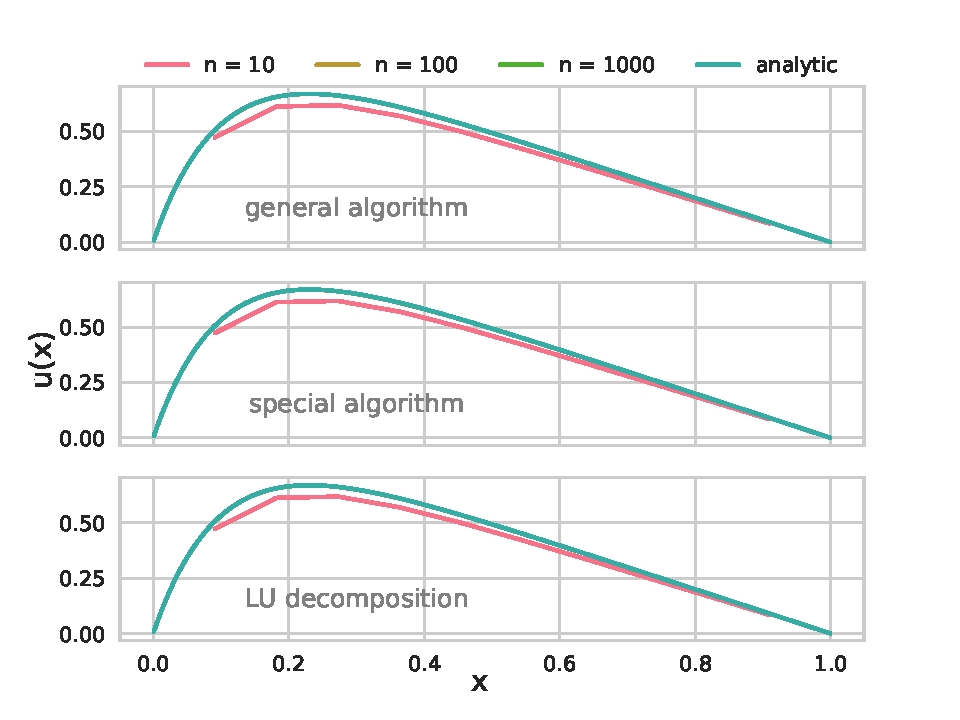
\includegraphics[width=\textwidth]{all_matrix_compare.pdf}
	\caption{We compare between unordered and ordered initial lattices, i.e. a random lattice and a lattice where all elements are set to 1.}
	\label{fig:unordered_ordered}
\end{figure}

\begin{figure}[htbp]
	\centering
	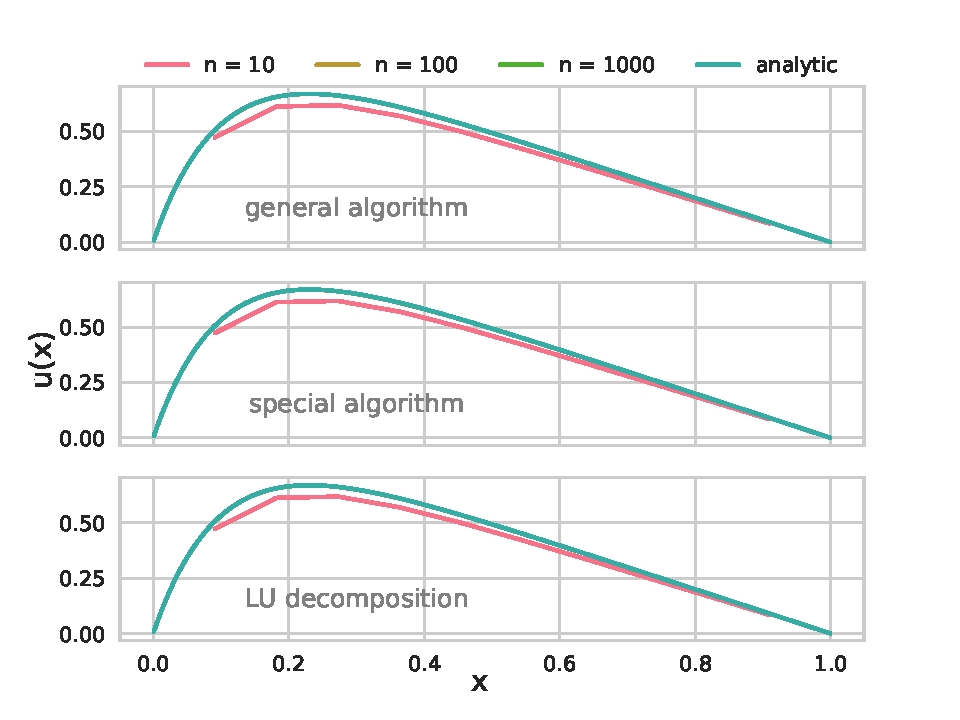
\includegraphics[width=\textwidth]{all_matrix_compare.pdf}
	\caption{Shown here is the probability distribution obtained from the Metropolis algorithm.}
	\label{fig:pde}
\end{figure}

\begin{figure}[htbp]
	\centering
	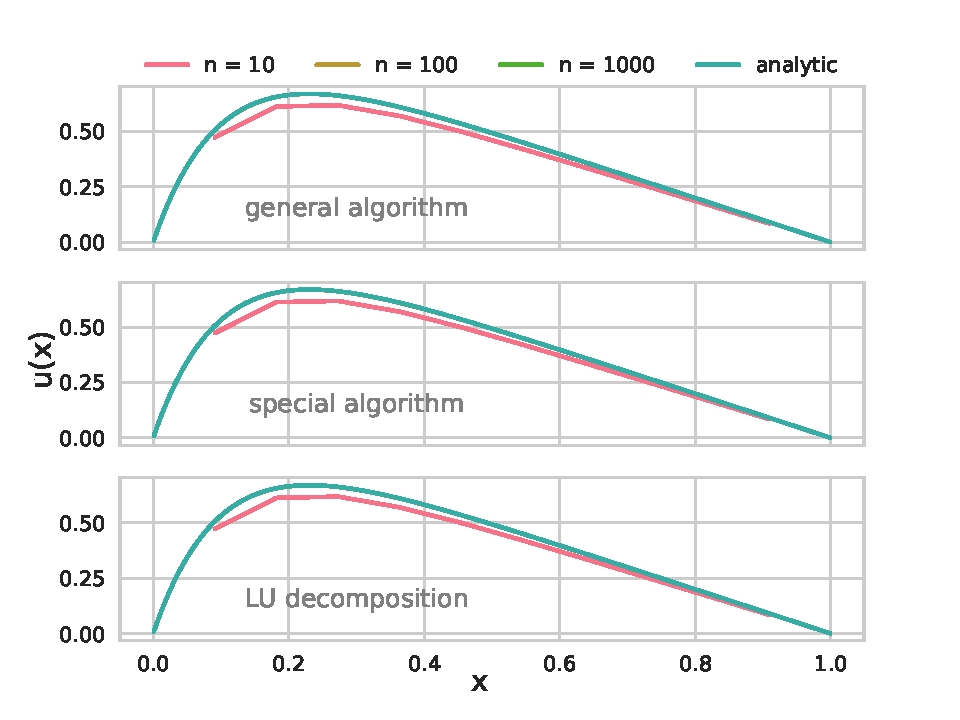
\includegraphics[width=\textwidth]{all_matrix_compare.pdf}
	\caption{Different parameters such as the expectation values of energy, magnetisation, specific heat capacity, and the susceptibility are here shown as a function of temperature ($[2.0, 2.3]$) for a selected lattice size, $L=100$.}
	\label{fig:phase_transition}
\end{figure}

\begin{figure}[htbp]
	\centering
	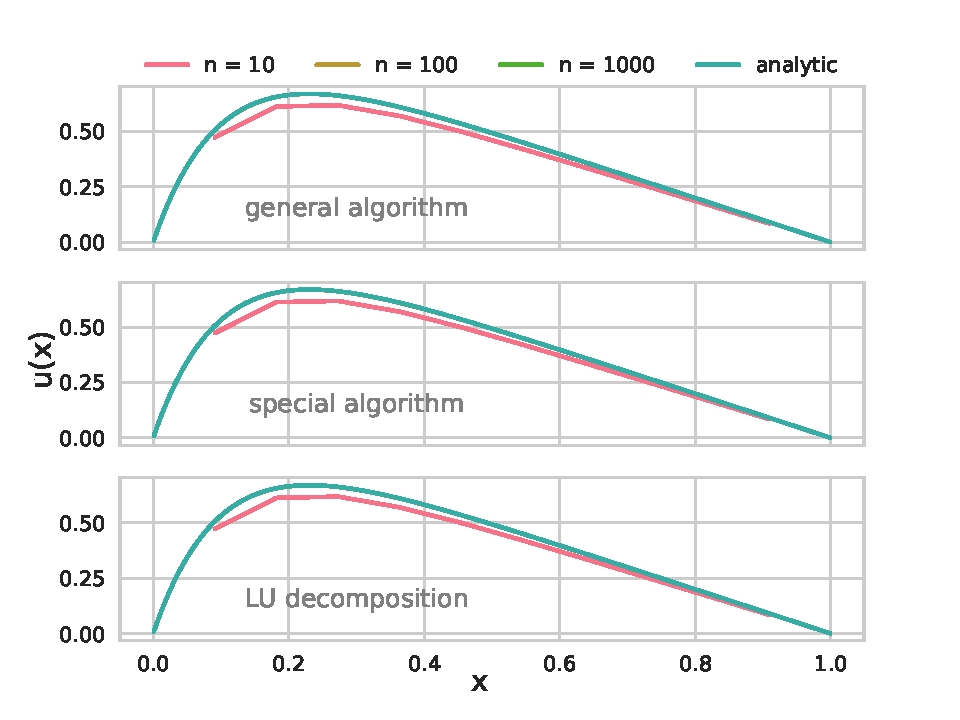
\includegraphics[width=\textwidth]{all_matrix_compare.pdf}
	\caption{Restricting the temperature domain to $[2.26, 2.30]$ we take a closer look at the heat capacity as a function of temperature for lattice sizes $L=40, 60, 80, 100$.}
	\label{fig:heatcap}
\end{figure}

\begin{table}[htbp]
	\centering
	\begin{tabular}{lrr}
		\textbf{n} & $\mathbf{{t_g}/{t_s}}$ & $\mathbf{{t_{LU}}/{t_s}}$  \\
		\midrule
		\addlinespace[0.1cm]

		10         & 2.08                                                                                          & 3.70                                                                                        \\
		$10^2$       & 1.89                                                                                          & $1.00\cdot 10^2 $                                                                                         \\
		$10^3$       & 1.48                                                                                          & $1.05 \cdot 10^4 $                                                                                        \\
		$10^4$       & 1.43                                                                                          & $1.18 \cdot 10^6$                                                                                         \\
		$10^5$       & 1.39                                                                                          & -                                                                                         \\
		$10^6$       & 1.41                                                                                          & -                                                                                        \\
		$10^7$       & 1.39                                                                                          &    -
	\end{tabular}  \caption{Ratio between CPU time for the general algorithm ($\mathbf{t_g}$), the special algorithm ($\mathbf{t_g}$) and the LU decomposition algorithm ($\mathbf{t_{LU}}$) for different matrix sizes (\textbf{n}). The LU decomposition crashed for \textbf{n} greater than $10^4$.} \label{table:time}
\end{table}
